\chapter{Trabalhos relacionados}

Neste capítulo são apresentados quatro sistemas de divulgação de vagas online em bolsas, estágios e empregos. O primeiro é a Plataforma de Gestão e Disseminação de Estágios Profissionais (PGDEP), uma aplicação Web para procura e divulgação de estágios profissionais entre alunos, diretores de cursos e empresas. O segundo é o Sistema de Gestão de Estágios e Empregos Online (SGEEO), que permite aos candidatos encontrar estágios e empregos através de processo de análise e seleção de currículos. O terceiro é a plataforma LinkedIn, uma rede social utilizada por profissionais para apresentarem suas aptidões. O quarto é o Mural de Bolsas, uma plataforma \textit{web} que facilita o preenchimento de vagas nas bolsas da UFRGS. Por fim, é realizada uma avaliação comparativa entre os quatro sistemas envolvendo critérios de funcionalidade e usabilidade.

\section{Plataforma de gestão e disseminação de estágios profissionais}
\label{trabRelPlatGestao}

A PGDEP \cite{PGDEPMono} foi implementada na Faculdade de Engenharia da Universidade do Porto, em Portugal, como proposta para melhorar o gerenciamento e indicação de estágios profissionalizantes mais adequados ao perfil dos alunos de cursos profissionalizantes. 

Entre as principais funcionalidades da plataforma estão:
\begin{itemize}
    \item Login no sistema;
    \item gerenciar alunos candidatos, diretor e coordenador de curso por escola;
    \item gerenciar empresas;
    \item gerenciar cursos;
    \item alunos podem pesquisar e se candidatarem a estágios;
    \item coordenador do curso cadastra Diretor do curso e cursos profissionais;
    \item diretor do curso lista alunos para estágio e monitora estágios ofertados pelas empresas;
    \item galeria de trabalhos realizados por alunos nos cursos;
    \item registro de competências adquiridas pelos alunos em estágios.
\end{itemize}

As Figuras \ref{telaHomePGDEP} e \ref{telaEscolaPGDEP} apresentam algumas das páginas presentes na PGDEP.

\begin{figure}[H]
    \caption{Tela inicial da PGDEP.}
       	\begin{center}
            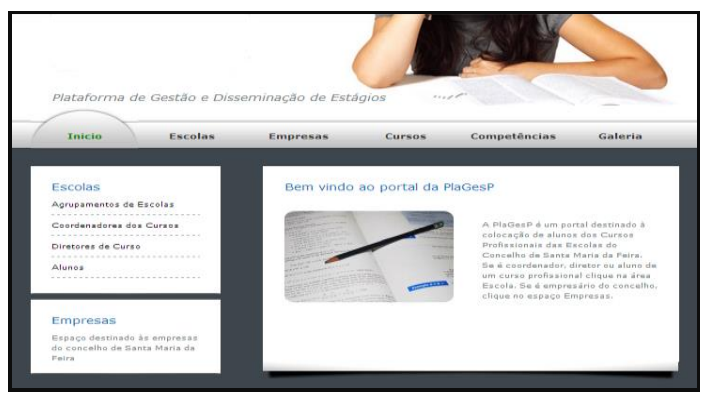
\includegraphics[width=0.75\textwidth]{figuras/rel03.png}
        \end{center}
    \label{telaHomePGDEP}
    \legend{Fonte: \cite{PGDEPMono}}
\end{figure}

\begin{figure}[H]
    \caption{Página de gestão das escolas cadastradas na plataforma PGDEP.}
       	\begin{center}
            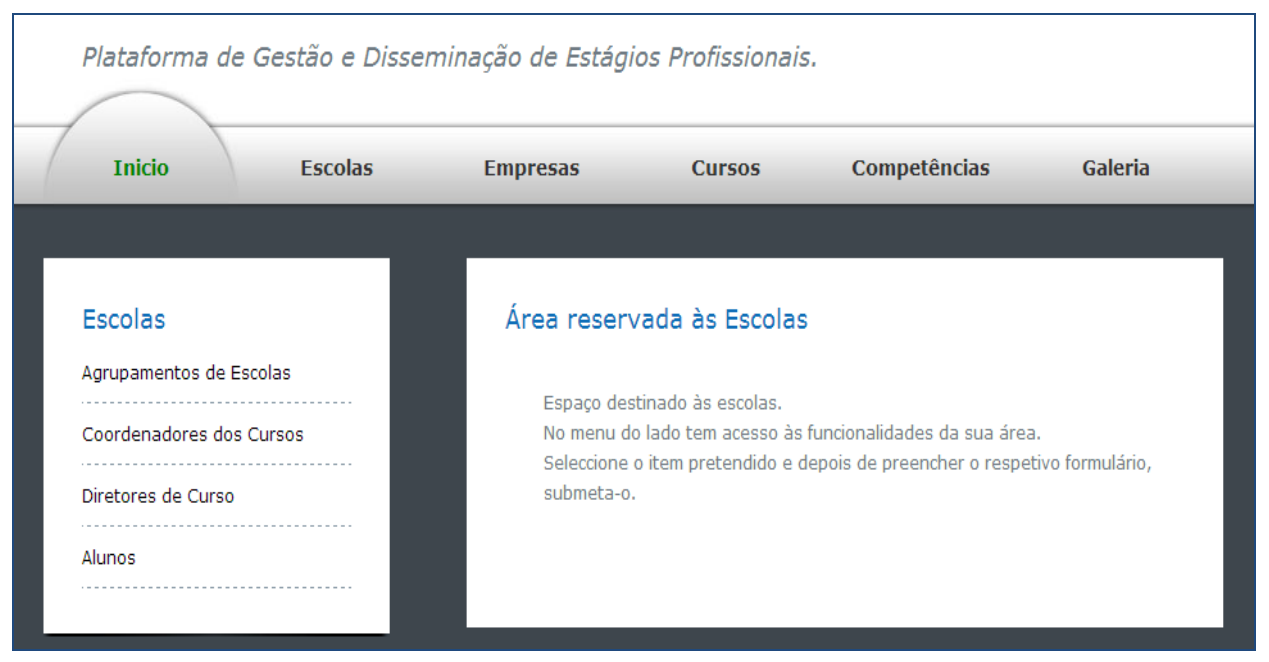
\includegraphics[width=0.75\textwidth]{figuras/rel04.png}
        \end{center}
    \label{telaEscolaPGDEP}
    \legend{Fonte: \cite{PGDEPMono}}
\end{figure}

A plataforma apresenta características interessantes como o \textit{feedback} do usuário após a experiência de estágio. Assim, empresas interessadas na contratação de um aluno terão um histórico deste de forma a complementar o processo de seleção. Adicionalmente, é possível receber recomendações do diretor, qualificando um candidato melhor preparado. Todavia, as interações entre os atores do sistema é bastante limitada, desestimulando interações entre usuários. Outras lacunas importantes da plataforma são a ausência de um sistema para favoritar vagas de interesse dos alunos, possibilidade de pesquisar usuários apenas para um grupo de atores e não ser possível o envio de currículos através do sistema.


\section{Sistema de gestão de estágios e empregos online}
\label{trabRelSistEmprego}

O SGEEO \cite{SGEEOMono} é um sistema desenvolvido na Universidade de Mindelo, no Cabo Verde, que objetiva aumentar o controle e a participação da Universidade com seus alunos no processo de pesquisa e seleção de estágios e empregos. A plataforma \textit{online} possibilita aos alunos cadastrarem seus currículos, selecionando sua área de interesse. As empresas parceiras, então, divulgam gratuitamente vagas de estágio ou emprego no sistema e os alunos interessados podem se inscrever e concorrer à vaga.

Entre as principais funcionalidades da plataforma estão:

\begin{itemize}
    \item Login no sistema;
    \item gerenciar candidatos e parceiros;
    \item candidatos podem enviar currículo, selecionar áreas de interesse e pesquisar vagas;
    \item parceiros podem pesquisar candidatos a partir da lista de currículos cadastrados no sistema;
    \item chat global para conversa entre usuários.
\end{itemize}

As Figuras \ref{telaHomeSGEEO} e \ref{telaCandidatoSGEEO} apresentam as telas inicial e de cadastro de currículo no SGEEO.

\begin{figure}[H]
    \caption{Tela inicial do SGEEO.}
       	\begin{center}
            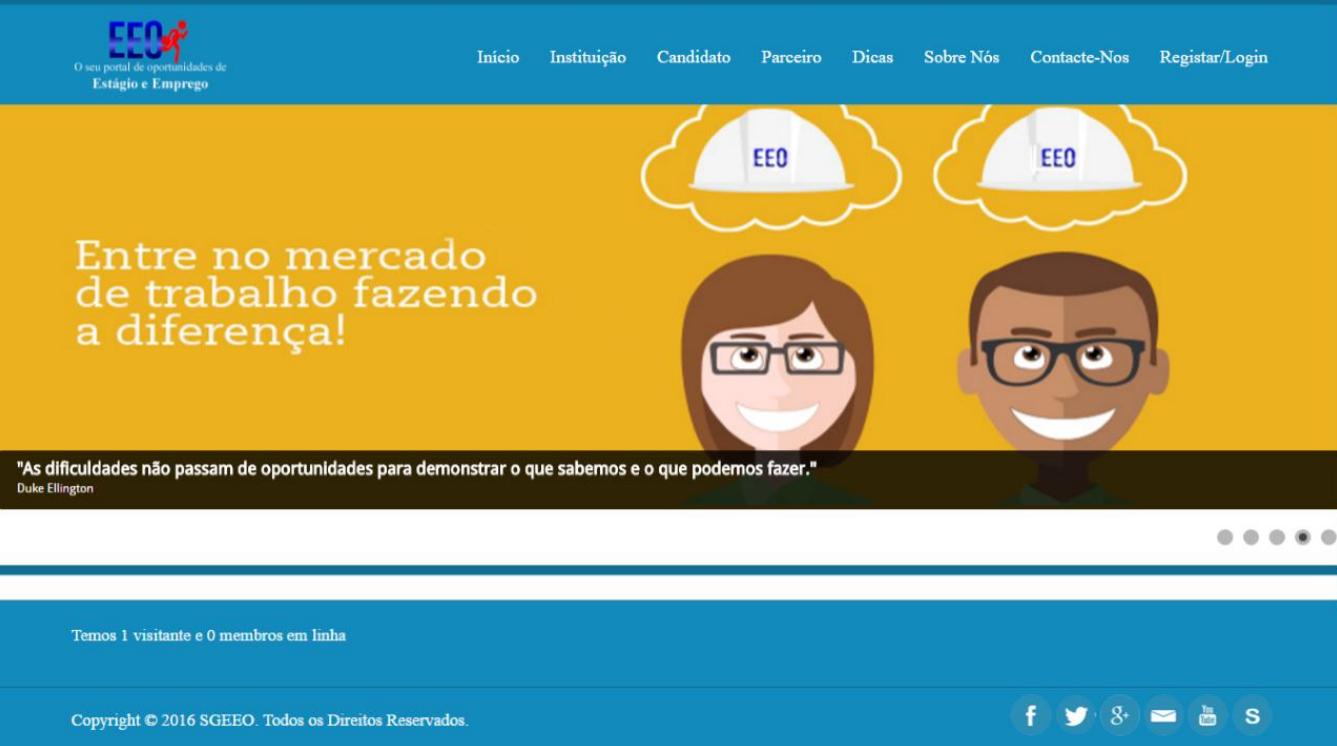
\includegraphics[width=0.75\textwidth]{figuras/rel01.png}
        \end{center}
    \label{telaHomeSGEEO}
    \legend{Fonte: \cite{SGEEOMono}}
\end{figure}

\begin{figure}[H]
    \caption{Tela de cadastro do currículo do candidato no SGEEO.}
       	\begin{center}
            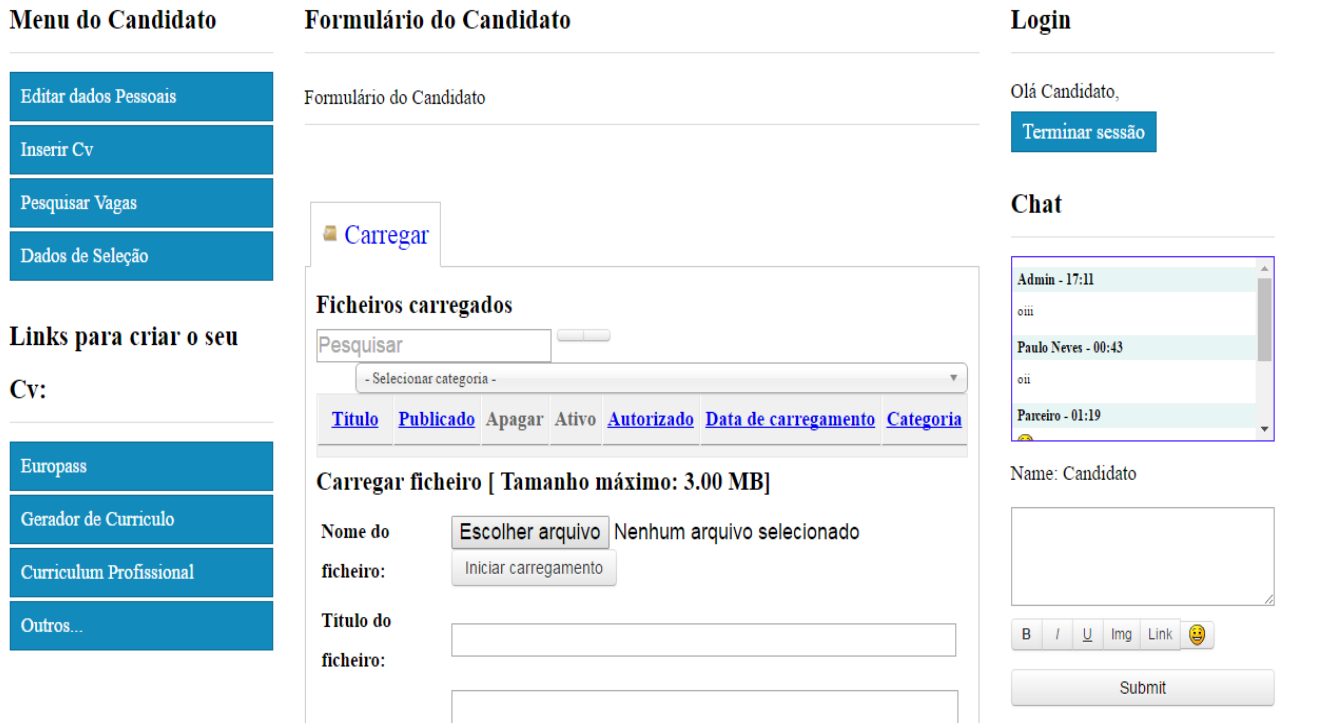
\includegraphics[width=0.75\textwidth]{figuras/rel02.png}
        \end{center}
    \label{telaCandidatoSGEEO}
    \legend{Fonte: \cite{SGEEOMono}}
\end{figure}

O SGEEO apresenta funcionalidades que propiciam maior interação entre os usuários do que o trabalho anterior. Há, adicionalmente, a possibilidade de envio de currículos e \textit{chat} entre usuários. O público-alvo do sistema aumentou: além de ofertar vagas em estágios, existem vagas para empregos. Entretanto, as funcionalidades de recomendações e \textit{feedbacks} de usuário foram depreciadas. Além disso, a pesquisa continua restrita a um grupo de usuários apenas e não há possibilidade de favoritar vagas de interesse para visualizar posteriormente de maneira mais rápida.

\section{LinkedIn}
\label{trabRelLinkedin}

LinkedIn\footnote{{\url{https://www.linkedin.com} Acesso em novembro de 2018}} é uma rede social voltada para negócios com grande destaque para o empreendedorismo e profissionais em geral. Através dele, usuários apresentam suas aptidões que são fortalecidas por recomendações de outros participantes da rede, promovendo interação e \textit{networking}. Além disso, é uma excelente plataforma para divulgação e pesquisa de vagas para as mais diversas categorias, incorporando desde estágios a programas de \textit{trainee} e, obviamente, de efetivo. A plataforma atualmente é a redes social de profissionais mais acessada e utilizada no mundo, contando com mais de 590 milhões de usuários\footnote{{\url{https://news.linkedin.com/about-us\#statistics} Acesso em novembro de 2018}}, sendo uma referência em termos de interação entre usuários, empresas e consequentes ofertas de emprego.

As principais funcionalidades da rede social são:
\begin{itemize}
    \item Login no sistema;
    \item curtir, comentar e compartilhar uma postagem;
    \item criar conexão com outro usuário;
    \item chat com usuários;
    \item pesquisar usuário e vagas;
    \item seguir usuários;
    \item recomendar usuário;
    \item criar artigos;
    \item ingressar em grupos de usuários;
    \item pesquisar, salvar, anunciar e compartilhar vagas;
    \item candidatar-se a vaga.
\end{itemize}

A Figura \ref{telaHomeLKDIN} apresenta a tela inicial da rede social LinkedIn após o usuário se autenticar no sistema.

\begin{figure}[h]
    \caption{Tela inicial de usuário no LinkedIn: \textit{feed} das pessoas e páginas que o usuário segue.}
       	\begin{center}
            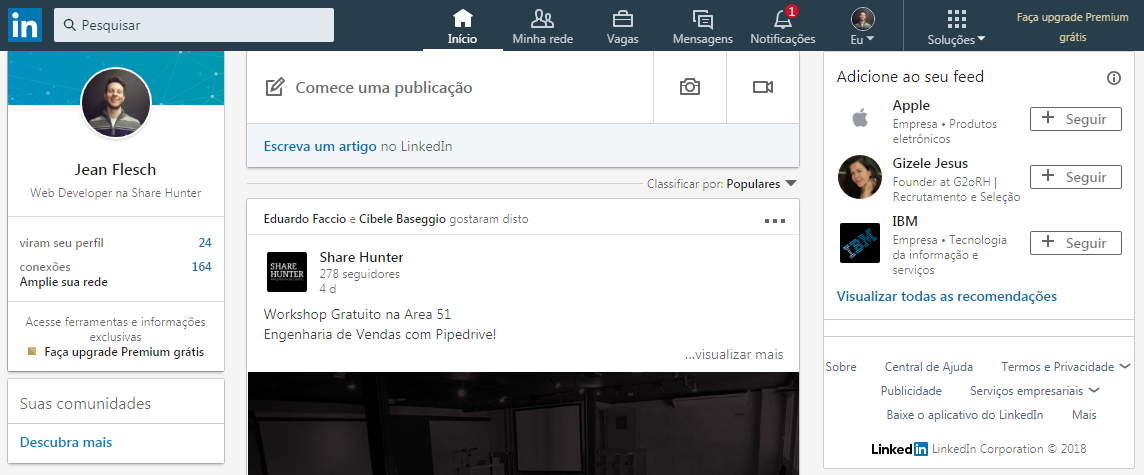
\includegraphics[width=0.85\textwidth]{figuras/rel05.png}
        \end{center}
    \label{telaHomeLKDIN}
    \legend{Fonte: LinkedIn}
\end{figure}

A plataforma LinkedIn é o exemplo perfeito de um ambiente que divulga vagas e promove uma interação constante entre seus usuários participantes. Todas as funcionalidades presentes -e ausentes- listadas nos trabalhos anteriores constituem a gama de opções que o LinkedIn oferece. Ainda, é possível realizar ações típicas e que cada vez mais são comuns em redes sociais, como curtir, compartilhar e comentar em uma postagem. Há a possibilidade de seguir, fazer amizades com e criar grupos de usuários também, aumentando o \textit{networking} entre os participantes. Apesar de todas suas qualidades, ele é uma solução independente da UFRGS. Portanto, todos os dados armazenados sobre alunos, professores, disciplinas ministradas e tantas outros não podem ser aproveitados, apesar do potencial da plataforma. Consequentemente, outras ferramentas que são utilizadas pela UFRGS também ficam prejudicadas com a eventual integração: o Moodle, Webmail, Portal da UFRGS, entre outros.

\section{Mural de Bolsas}
\label{trabRelMDB}

O MB\footnote{{\url{https://www.ufrgs.br/bolsas/}, Acesso em novembro de 2018}} é um portal online disponível para uso na UFRGS. Desenvolvido pela Empresa Jr. IDE\footnote{{\url{https://idejr.com.br/}, Acesso em novembro de 2018}}, composta por alunos de graduação de diferentes cursos e áreas de conhecimento na Universidade. A proposta da plataforma foi reformar o antigo sistema da própria UFRGS que simplesmente divulgava uma tabela precária, com poucas informações sobre as vagas disponíveis em bolsas. 

Com a reestruturação do site e, consequente construção do portal, a experiência de usuário aumentou drasticamente  com a inclusão de várias funcionalidades. Entre elas, estão:
\begin{itemize}
    \item Login no sistema integrado com banco de dados da UFRGS;
    \item alunos podem pesquisar vagas;
    \item administradores podem gerenciar vagas;
    \item enviar e-mail com atualizações periódicas;
    \item configurar opções da conta de usuário.
\end{itemize}

As Figuras \ref{telaHomeMB} e \ref{telaVagasMB} apresentam algumas das telas da plataforma do Mural de Bolsas.

\begin{figure}[H]
    \caption{Página inicial do MB com informações do portal para alunos e professores.}
       	\begin{center}
            
\includegraphics[width=0.68\textwidth]{figuras/rel06.png}
        \end{center}
    \label{telaHomeMB}
    \legend{Fonte: Empresa Jr. IDE}
\end{figure}

\begin{figure}[H]
    \caption{Tela de exibição das vagas disponíveis do portal do MB para alunos pesquisarem bolsas.}
       	\begin{center}
            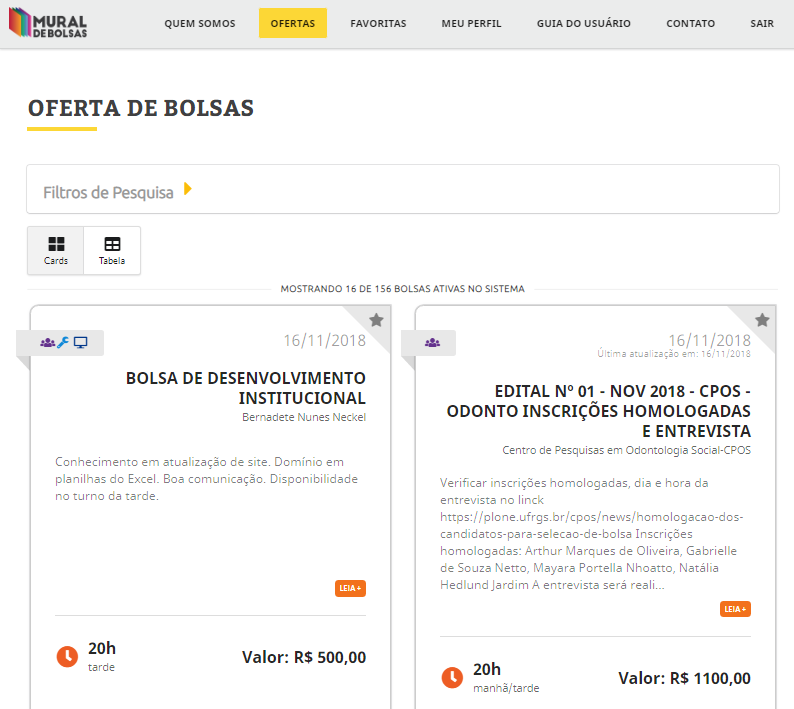
\includegraphics[width=0.68\textwidth]{figuras/rel07.png}
        \end{center}
    \label{telaVagasMB}
    \legend{Fonte: Empresa Jr. IDE}
\end{figure}

O Mural de Bolsas é uma ferramenta que propicia uma lista de vagas em bolsas na UFRGS onde alunos podem filtrar por termos de interesse e campos pré-definidos da base de dados. É uma maneira prática e simples de apresentar um repositório de vagas. As bolsas são cadastradas por administradores do sistema e todos os usuários possuem uma conta de usuário dentro da UFRGS. Portanto, este é um exemplo de sistema integrado, tangenciando um dos objetivos deste trabalho. No entanto, ele possui limitações que precisam ser observadas. 

A primeira delas é a própria integração: basicamente, ela serve apenas para permitir que usuários autenticados acessem as listas de vagas, internas ao sistema; não há um registro ou mesmo utilização de informações oriundas de outras ferramentas da Universidade. Pode-se citar também que o sistema oferece poucas ações: pesquisa, filtro e uma configuração bastante simples das preferências de usuário. Mesmo a proposta sendo simples, ela apresenta lacunas como a falta de critérios de ordenação dos resultados exibidos, filtros um pouco mais complexos e uma melhor gerência de vagas favoritadas. É notório também que a experiência de usuário é levemente abalada com a ausência de algumas funcionalidades auxiliares, como não existir \textit{links} para contato direto com o autor da vaga, por exemplo.

\section{Análise comparativa}
\label{trabRelAnalise}

Através da análise das soluções das seções prévias, percebe-se muitas funcionalidades semelhantes e outras que divergem por apresentarem propostas e regras de negócio diferentes. Com o objetivo de agrupar as funcionalidades mais comuns nas plataformas e compará-las, será apresentada uma tabela com as principais características que se acredita ser um diferencial em sistemas de recomendação de vagas. 

\begin{table}[h]
    \begin{adjustwidth}{-0.7in}{-0.7in}
    \begin{center}
    \caption{Tabela comparativa sobre os trabalhos relacionados}
    \begin{tabular}{>{\columncolor{tableblue!30}}l|l|l|l|l|l}
        \hline
        \rowcolor{tableblue}
                            & \textbf{PDGEP}  & \textbf{SGEEO}    & \textbf{LKDIN}& \textbf{MB} \\
        \hline
    \textit{Software}   & Sistema         & Sistema           & Rede social   & Sistema \\
    Oferta              & Estágios        & Estágios, empregos &Estágios, empregos & Bolsas \\
    Login               & Sim             & Sim               & Sim           & Sim \\
    Enviar currículo    & Não             & Sim               & Sim           & Não \\
    Pesquisar vagas     & Sim             & Sim               & Sim           & Sim \\
    Pesquisar usuários  & Apenas empresas & Apenas parceiros  & Sim           & Não \\
    Candidatar-se a vaga& Sim             & Sim               & Sim           & Não \\
    \textit{Feedback} do candidato & Sim  & Não               & Sim           & Não \\
    Preferências do usuário & Sim         & Sim               & Sim           & Sim \\
    Recomendações       & Sim             & Não               & Sim           & Não \\
    Favoritar vagas     & Não             & Não               & Sim           & Sim \\
    Seguir usuário      & Não             & Não               & Sim           & Não \\
    Amizades            & Não             & Não               & Sim (conexões) & Não \\
    Fazer posts         & Não             & Não               & Sim           & Não \\
    Fazer comentários   & Não             & Não               & Sim           & Não \\
    Compartilhar vagas  & Não             & Não               & Sim           & Não \\
    Grupos de usuários  & Não             & Não               & Sim           & Não \\
    Chat Online         & Não             & Global            & Individual    & Não \\
    \hline
    
    \end{tabular}
    \end{center}
    \end{adjustwidth}
    \bigskip
    \legend{Tabela com as principais funcionalidades dos quatro sistemas apresentados neste capítulo. A sigla LKDIN significa LinkedIn. }
    \label{tabelaAvalTrab}
\end{table}

Os trabalhos apresentadas possuem características únicas, mas que convergem a um objetivo principal: facilitar a divulgação (direta ou indireta) de vagas em diversos tipos de trabalho. Os trabalhos PDGEP e SGEEO são bastante próximos, divergindo em alguns pontos como nicho de ofertas de emprego e a questão de recomendação e \textit{feedback} do candidato (PGDEP) contra uma maior interação entre os usuários via preenchimento e envio de currículo e \textit{chat} (SGEEO). A rede social LinkedIn é a mais completa, apresentando todos os recursos considerados fundamentais para uma aplicação interativa e informativa; porém, é importante ressaltar a complexidade de desenvolver uma ferramenta tão completa e robusta como essa. O Mural de Bolsas, por sua vez, possui uma integração com a base de dados da UFRGS e foca a divulgação de suas ofertas totalmente no âmbito acadêmico, através da divulgação de bolsas administrativas e de iniciação científica.

Considerando as peculiaridades de cada sistema, é proposto neste trabalho, a elaboração de um protótipo de rede social que cubra os principais pontos enumerados neste capítulo. A possibilidade de envio de currículos, pesquisar e recomendar usuários e vagas para todos atores do sistema, candidatar-se e favoritar uma vaga, seguir usuários, fazer comentários, postagens e curti-las, preencher seu próprio perfil e facilidade na divulgação de ofertas de vagas em estágios, bolsas acadêmicas e empregos são funcionalidades consideradas importantes para alcançar o objetivo de desenvolver uma plataforma interativa e de fácil gestão, utilização e manutenção. 